% Feel free to contact me for any reason:
%% Email 1: zain.kamal@rutgers.edu
%% Email 2: z.kamal2021@gmail.com
%% Discord: alci#6038

%%%%%%%%%%%%%%%%%%%%%%%%%%%%%%%%%%%%%%%%%%%%%%%%%%%%%%%%%%%%%%%%%%%%%%%%%%%%%%%%%
\documentclass{article}
% Feel free to contact me for any reason:
%% Email 1: zain.kamal@rutgers.edu
%% Email 2: z.kamal2021@gmail.com
%% Discord: alci#6038

% Last updated 1/28/22

% Template based off of Justin Kim's (don't know where he got it from originally), but I've made a ton of edits. His soul lives on in random packages and commands I'm too lazy to comment out.


%%%%%%%%%%%%%%%%%%%%%%%%%%%%%%%%%%%%%%%%%%%%%%%%%%%%%%%%%%%%%%%%%%%%%%%%%%%%%%%%%%%%
%%% Default packages:

\usepackage[margin=1in]{geometry} 
\usepackage{amsmath,amsthm,amssymb,amsfonts, fancyhdr, color, comment, graphicx, environ}
\usepackage{xcolor}
\usepackage{mdframed}
\usepackage{bm}
\usepackage[shortlabels]{enumitem}
\usepackage{mathtools}
\usepackage{listings}
\usepackage{stmaryrd}
\usepackage{indentfirst}
\usepackage{hyperref}


%%%%%%%%%%%%%%%%%%%%%%%%%%%%%%%%%%%%%%%%%
%%% Pacakages I've added:

%% For Math 300 (Winter 2021):

\usepackage{mathdots} % for \iddots

\usepackage[ruled]{algorithm2e} % Algorithms
% NOTE: FIND A BETTER ALGORITHM PACKAGE, OR ATLEAST LEARN HOW TO USE THIS ONE BECAUSE DOUBLE INDENTING IS A FUCKING NIGHTMARE (or just import from mathcha?)
%% Example algorithm:
% \begin{center}
% 	\begin{minipage}{0.5\linewidth} % Adjust the minipage width to accomodate for the length of algorithm lines
% 		\begin{algorithm}[H]
% 			\KwIn{$(a, b)$, two floating-point numbers}  % Algorithm inputs
% 			\KwResult{$(c, d)$, such that $a+b = c + d$} % Algorithm outputs/results
% 			\medskip
% 			\If{$\vert b\vert > \vert a\vert$}{
% 				exchange $a$ and $b$ \;
% 			}
% 			$c \leftarrow a + b$ \;
% 			$z \leftarrow c - a$ \;
% 			$d \leftarrow b - z$ \;
% 			{\bf return} $(c,d)$ \;
% 			\caption{\texttt{FastTwoSum}} % Algorithm name
% 			\label{alg:fastTwoSum}   % optional label to refer to
% 		\end{algorithm}
% 	\end{minipage}
% \end{center}



%%%%%%%%%%%%%%%%%%%%%%%%%%%%%%%%%%%%%%%%%%%%%%%%%%%%%%%%%%%%%%%%%%%%%%%%%%%%%%%%%%%%
%%% Default commands:

\renewcommand{\vec}[1]{\mathbf{#1}}
	
\newcommand{\WidestEntry}{$lon_1$}%
\newcommand{\SetToWidest}[1]{\makebox[\widthof{\WidestEntry}]{#1}}%
\newcommand\tab[1][0.61cm]{\hspace*{#1}}
\newcommand{\nats}{\mathbb{N}}
\newcommand{\rats}{\mathbb{Q}}
\newcommand{\reals}{\mathbb{R}}
\newcommand{\Z}[1]{\mathbb{Z}_{#1}}
\newcommand{\BigO}[1]{\mathcal{O}(#1)}
\newcommand{\seq[1]}{(#1_n)}
\newcommand{\subseq[1]}{(#1_{n_k})}
\newcommand{\Lim}[2]{\lim \limits _{#1 \to #2}}
\newcommand{\Min}[2]{\min \{#1, #2\}}
\newcommand{\inv}{^{-1}}
\newcommand{\h}{^\text{th}}
\newcommand{\lrangle}[1]{\langle #1 \rangle}
\newcommand{\abs}[1]{\left\lvert #1 \right\rvert}

\DeclarePairedDelimiter{\ceil}{\lceil}{\rceil}
\DeclarePairedDelimiter{\floor}{\lfloor}{\rfloor}
\DeclareMathOperator{\supp}{supp}
\DeclareMathOperator{\rad}{rad}
\DeclareMathOperator*{\argmin}{arg\,min}
\DeclareMathOperator*{\argmax}{arg\,max}
\DeclareMathOperator*{\Var}{Var}
\DeclareMathOperator*{\Cov}{Cov}
\DeclareMathOperator*{\Corr}{Corr}
\DeclareMathOperator*{\Aut}{Aut}
\newcommand{\prob}[1]{\section*{Problem #1}}


%%%%%%%%%%%%%%%%%%%%%%%%%%%%%%%%%%%%%%%%%
%%% Commands I've added:

%% For Math 300 (Winter 2021):

\newcommand{\lrbrace}[1]{\{ #1 \}}
\newcommand{\powerset}{\mathcal{P}}
\newcommand{\ints}{\mathbb{Z}}

% Source/inspiration: https://tex.stackexchange.com/a/42728:
\newcommand{\numberthis}{\addtocounter{equation}{1}\tag{\theequation}\label{\theequation}}
    % Within an `align*` environment, put `\numberthis` after a line to number it. 
    % Access it with `\eqref{ [number of equation] }`
\newcommand{\numberthiswith}[1]{\addtocounter{equation}{1}\tag{\theequation}\label{#1}}
    % Within an `align*` environment, put `\numberthiswith{ [your_label] }` after a line to number it. 
    % Access it with `\eqref{ [your_label] }`



%%%%%%%%%%%%%%%%%%%%%%%%%%%%%%%%%%%%%%%%%%%%%%%%%%%%%%%%%%%%%%%%%%%%%%%%%%%%%%%%%%%%
%%% Default formatting:

\hypersetup{
    colorlinks=true,
    linkcolor=blue,
    filecolor=magenta,      
    urlcolor=blue,
}

\setlength{\parindent}{0cm}
\setlength{\parskip}{6pt}

\pagestyle{fancy}


%% Misc formatting additions

% make bullets with itemize much smaller
\newlength{\mylen}
\setbox1=\hbox{$\bullet$}\setbox2=\hbox{\tiny$\bullet$}
\setlength{\mylen}{\dimexpr0.5\ht1-0.5\ht2}
\renewcommand\labelitemi{\raisebox{\mylen}{\tiny$\bullet$}}


% Modified version of problem environment below
% \newenvironment{problem}[2][Problem]
%     { \begin{mdframed}[backgroundcolor=gray!5] \textbf{#1 #2} \\}
%     {  \end{mdframed}}
% \newenvironment{solution}{\textbf{Solution}\\}


%%%%%%%%%%%%%%%%%%%%%%%%%%%%%%%%%%%%%%%%%
%%% Formatting I've added:

%% Grey boxes for problem statements (note that I don't have a "solution" section):

% Problem environment, but shows "(a)" instead of "Problem a"
\newenvironment{problem}[2][]
    { \begin{mdframed}[backgroundcolor=gray!5] \textbf{#1 (#2)}}
    {  \end{mdframed}}
% Problem environment, but no "([input_char])" at all
\newenvironment{problem*}
    { \begin{mdframed}[backgroundcolor=gray!5] \\}
    {  \end{mdframed}}


% Example environment, currently identical to "problem" (Note: this is better written than the problem environment because I wrote it myself from scratch. Use this as an example for future new environments.)
\newcounter{example}[section]
\newenvironment{example}
    { 
        \refstepcounter{example}
        \begin{mdframed}[backgroundcolor=gray!5]
        \textbf{\\Example \thesection.\theexample:}
    }
    {\\ \end{mdframed}}


%%%%%%%%%%%%%%%%%%%%%%%%%%%%%%%%%%%%%%%%%%%%%%%%%%%%%%%%%%%%%%%%%%%%%%%%%%%%%%%%%%%%
% Misc things I've added




%%%%%%%%%%%%%%%%%%%%%%%%%%%%%%%%%%%%%%%%%%%%%
% Fill in the appropriate information below
\lhead{Zain Kamal}
% \rhead{Math 244 Spring 2022} % Moved to document
% \chead{\textbf{Homework 2}} % Moved to document
\begin{document}
\chead{\textbf{Physics 228: HW 1 Notes}}
\rhead{1/30/22}
%%%%%%%%%%%%%%%%%%%%%%%%%%%%%%%%%%%%%%%%%%%%%%%%%%%%%%%%%%%%%%%%%%%%%%%%%%%%%%%%%

\textbf{\underline{(1)}}
\begin{equation*}
v=\vec{E} \times \vec{B}
\end{equation*}

\

\hline

\textbf{\underline{(2-3)}}

high index of refraction $\Longleftrightarrow $ more aligned with normal

\

\hline

\textbf{\underline{(4)}}

\begin{example}

What inductance must be connected to a 18 pF capacitor in an oscillator capable of generating 600 nm (i.e., visible) electromagnetic waves? Comment on your answer.

\end{example}



Relating frequency and wavelength of EM wave:
\begin{equation*}
\boxed{c=f\lambda } .
\end{equation*}


Frequency of oscillation of current in LC circuit:
\begin{equation*}
\boxed{f=T^{-1} =\frac{1}{2\pi \sqrt{LC}}} .
\end{equation*}
Thus:
\begin{align*}
2\pi \sqrt{LC} & =\frac{\lambda }{c} .
\end{align*}
\textit{Note: }$c=3\times 10^{8} \ m/s$.



My mistake was forgetting that $T=\frac{1}{f}$.


\


\hline

\textbf{\underline{(5)}}

\begin{example}

What is the intensity of a traveling plane electromagnetic wave if Bm is 4.8 ✕ 10−4 T?

\end{example}



"Intensity" = Average of the Poynting vector:
\begin{align*}
I=\langle S\rangle  & =\frac{1}{2\mu _{0}} E_{0} B_{0}
\end{align*}
\textit{Note: }$\mu _{0} =1.26\times 10^{-6} \ H/m$.


\


\hline

\textbf{\underline{(6)}}

Power is given by:
\begin{align*}
\Aboxed{P & =\frac{E}{\Delta t}} .
\end{align*}


Not needed for this problem, but energy of a photon is given by:
\begin{align*}
E & =hf\\
 & =h\frac{c}{\lambda } .
\end{align*}
\textit{Note: }$h=6.626\times 10^{-34} \ J\cdot s$

\



\hline

\textbf{\underline{(7)}}

Imagine a source of power is radiating waves isotropically, which means equally in all directions. At a distance $r$, all of the radiated power is radiated through a sphere with area $4\uppi r^{2}$. So the intensity at $r$ from the source is:
\begin{equation*}
\boxed{I=\frac{P}{A} =\frac{P}{4\pi r^{2}}} .
\end{equation*}

\begin{figure}[htp]
    \centering
    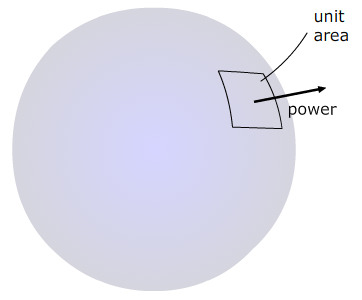
\includegraphics[width=6cm]{images/hw1.1.png}
\end{figure}


\begin{figure}[htp]
    \centering
    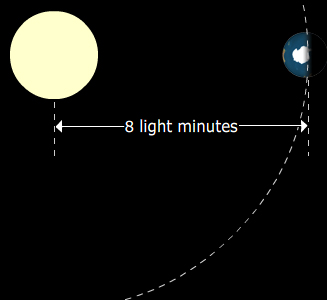
\includegraphics[width=6cm]{images/hw1.2.png}
\end{figure}

\textit{\href{https://www.animations.physics.unsw.edu.au/jw/waves\_power.htm}{(Source)}}


\


\hline

\textbf{\underline{(11)}}

Critical angle is the angle of incidence that provides an angle of refraction of 90-degrees:
\begin{equation*}
\boxed{\theta _{crit} =\sin^{-1}\left(\frac{n_{2}}{n_{1}}\right)} .
\end{equation*}
Note: be careful about where the ray is originating from when assigning $n_{2}$ and $n_{1}$.


\clearpage
\

\hline

\textbf{\underline{(12)}}

\begin{figure}[htp]
    \centering
    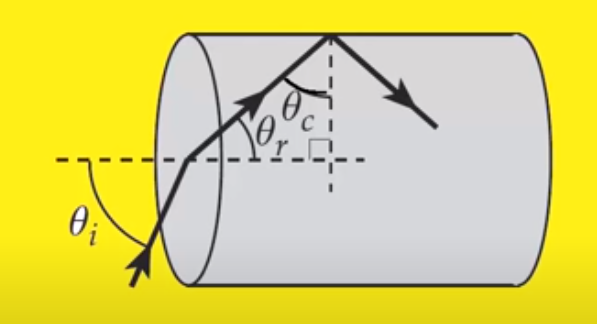
\includegraphics[width=6cm]{images/hw1.3.png}
\end{figure}

$\theta _{c}$ represents the critical angle where any transmitted light is parallel to the surface ($\theta _{t} =90$). Effectively, this means that all light is reflected:
\begin{equation*}
\theta _{c} =\sin^{-1}\left(\frac{n_{outside}}{n_{inside}}\right) .
\end{equation*}
From the right angle, we easily see:
\begin{equation*}
\theta _{r} =90-\theta _{c} .
\end{equation*}
Finally, we find $\theta _{i}$ with Snell's Law:
\begin{equation*}
\theta _{i} =\sin^{-1}\left(\frac{n_{inside}\sin \theta _{r}}{n_{outside}}\right) .
\end{equation*}








%%%%%%%%%%%%%%%%%%%%%%%%%%%%%%%%%%%%%%%%%%%%%%%%%%%%%%%%%%%%%%%%%%%%%%%%%%%%%%%%%
\end{document}